\documentclass[10pt,letterpaper]{article}

% --- Packages ---
\usepackage[utf8]{inputenc}
\usepackage[T1]{fontenc}
\usepackage[hidelinks]{hyperref}
\usepackage{geometry}
\usepackage{parskip}
\usepackage{titlesec}
\usepackage{enumitem}
\usepackage{xcolor}
\usepackage{amssymb}
\usepackage{amsmath}
\usepackage{booktabs}
\usepackage{tabularx}
\usepackage{tikz}
\usepackage{tcolorbox}
\usepackage{microtype}
\usetikzlibrary{shapes.geometric, arrows.meta, positioning, fit, backgrounds, calc}

% --- Global Color & Formatting Setup ---
\titleformat{\section}{\normalsize\bfseries\color{black!85}}{}{0pt}{}[\vspace{-4pt}\color{black!15}\rule{\textwidth}{0.3pt}\vspace{-1pt}]
\titlespacing{\section}{0pt}{10pt}{3pt}
\titleformat{\subsection}{\small\bfseries}{}{0pt}{}
\titlespacing{\subsection}{0pt}{6pt}{2pt}

\newlist{tightemize}{itemize}{1}
\setlist[tightemize]{label=$\bullet$, leftmargin=15pt, topsep=1pt, itemsep=1pt, parsep=0pt}

\definecolor{csblue}{RGB}{59,130,246}
\definecolor{csgreen}{RGB}{34,197,94}
\definecolor{csred}{RGB}{239,68,68}
\definecolor{csorange}{RGB}{249,115,22}
\definecolor{cspurple}{RGB}{139,92,246}
\definecolor{csbg}{RGB}{248,250,252}

\setlength{\parskip}{2pt}
\setlength{\parindent}{0pt}

\begin{document}

% ==========================================
% PAGE 1: COVER (title + GitHub repo only)
% ==========================================
\newgeometry{left=0.6in, top=0.5in, right=0.6in, bottom=0.5in}

\vspace*{2.0cm}

\begin{center}
    {\Huge \textbf{CivicSync}}\\[10pt]
    {\LARGE Intelligent Emergency Response}\\[2pt]
    {\LARGE \& Resource Optimization Platform}\\[20pt]

    \rule{0.5\textwidth}{0.5pt}\\[14pt]

    {\Large \textbf{Problem Statement}}\\[16pt]

    \begin{tcolorbox}[colback=csbg, colframe=csblue, boxrule=0.6pt, arc=4pt,
        left=12pt, right=12pt, top=10pt, bottom=10pt,
        width=0.85\textwidth]
    \large
    \textbf{Submission ID:} PSTU-HACK-2026-0102\\[4pt]
    \textbf{Track:} Backend Architecture \& Decision-Making Engine\\[4pt]
    \textbf{GitHub Source Code:} \\
    \texttt{\href{https://github.com/AhmedTrooper/Civic-Sync}{https://github.com/AhmedTrooper/Civic-Sync}}
    \end{tcolorbox}
\end{center}

\clearpage

% ==========================================
% PAGE 2: ABSTRACT
% ==========================================

\begin{tcolorbox}[colback=csbg, colframe=csblue, boxrule=0.6pt, arc=3pt,
    left=8pt, right=8pt, top=6pt, bottom=6pt, title=\textbf{Abstract (250 words)},
    fonttitle=\bfseries]
\small
We present \textbf{CivicSync}, a backend that turns fragmented national emergency response into one ranked, coordinated, explainable grid. Eight divisional command centers --- Dhaka as Core plus seven regional hubs --- share a single dispatch fabric that re-optimises continuously as incidents, road closures, vehicle failures, and capacity changes arrive.

\textbf{Architecture.} Rust/Axum 0.8 + Tokio ships as one static binary with sub-millisecond p50 latency; sqlx delivers compile-checked PostgreSQL with PostGIS; Redis supplies a 60-second nearest-center cache with quantised 4-decimal keys ($\sim$11 m). The TanStack dashboard consumes a 60-second conditional flush over WebSocket --- idle periods produce zero traffic.

\textbf{Decision engine.} A deterministic multi-center planner ranks incidents by a priority score (severity $\times$ 10 + casualties $\times$ 0.5 + affected $\times$ 0.02 + time-on-grid), then layers primary hub $\rightarrow$ Dhaka Core $\rightarrow$ regional hubs, capped at three assets per incident. Double-allocation is impossible: a \texttt{HashSet} claimed-set in planning \emph{and} an \texttt{assigned\_incident\_id IS NULL} row guard under \texttt{FOR UPDATE} at commit.

\textbf{AI.} A provider-agnostic Rig orchestrator (OpenAI, Anthropic, Gemini, DeepSeek, Cohere, Ollama) refines per-envelope justification text only --- never the allocation. A tokio semaphore enforces 3 LLM calls per 30 s; overflow degrades to the heuristic and increments a Prometheus counter.

\textbf{Reliability.} Every external dependency is optional. With no \texttt{DATABASE\_URL} the API boots in-memory (\texttt{Arc<Mutex<HashMap>>}); without Redis, Haversine computes directly; without an AI key, the heuristic runs identically. The same router, same semantics, same wire contract.

\textbf{Verification.} Four-layer gate: cargo check + clippy + fmt, 12-stage live smoke, frontend body contract, Zod schema contract --- all green under one command.
\end{tcolorbox}

% ==========================================
% PAGE 3: PROBLEM ANALYSIS & ARCHITECTURE
% ==========================================
\clearpage

\section{Problem Analysis}
The platform must continuously receive emergency incidents from multiple regions while coordinating ambulances, hospitals, rescue teams, helicopters, and emergency operation centers. Each incident carries geographic location, severity, affected population, time sensitivity, resource requirements, and environmental conditions; each resource carries live location, availability, capacity, ETA, operational constraints, and failure state. The environment changes non-stop: new requests, road closures, hospitals at capacity, vehicle failures, communication delays. Decisions must be near-optimal, explainable, operationally feasible, and adaptive in near real time.

\begin{tcolorbox}[colback=csbg, colframe=csgreen, boxrule=0.5pt, arc=3pt,
    left=8pt, right=8pt, top=4pt, bottom=4pt, title=\textbf{Why this is hard},
    fonttitle=\bfseries\small]
\footnotesize
\textbf{1. Conflict freedom.} Two incidents may simultaneously need the same ambulance; the system must guarantee --- not probabilistically mitigate --- that one asset is never promised twice. \textbf{2. Live re-planning.} A resource that flips to \texttt{STUCK} mid-route must be re-routed within the next decision cycle, not the next hour. \textbf{3. Graceful degradation.} When the network drops or the LLM throttles, dispatch must continue with the same wire contract --- operators in the field cannot wait for a retry. \textbf{4. Explainability.} Every allocation decision must be auditable by a human reviewer using the same arithmetic the engine used, regardless of whether an LLM was involved.
\end{tcolorbox}

\section{Overall System Architecture}

\begin{center}
\scalebox{1.18}{%
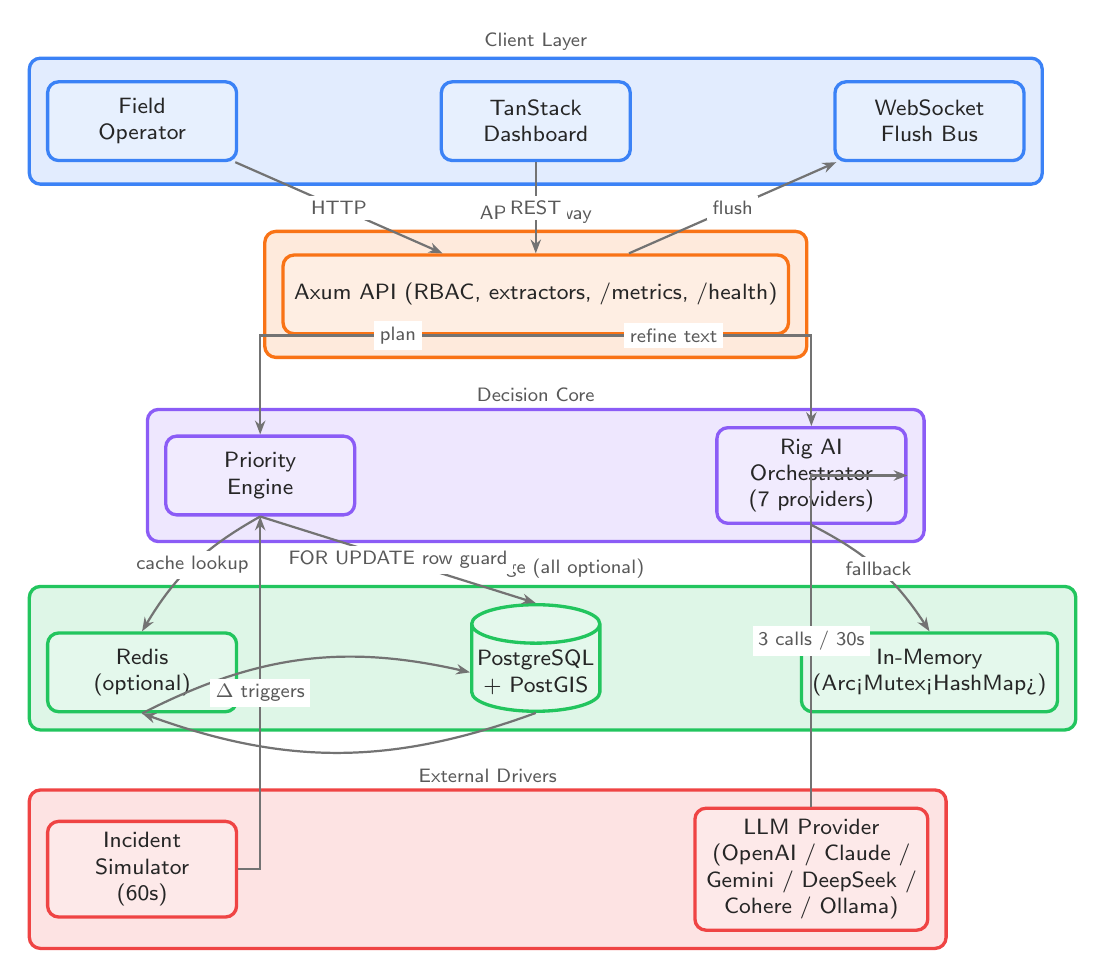
\begin{tikzpicture}[
    font=\sffamily\footnotesize,
    box/.style={rectangle, rounded corners=4pt, draw=#1, very thick, fill=#1!12,
                minimum width=2.4cm, minimum height=1cm, align=center, inner sep=4pt, text=black!85},
    db/.style={cylinder, shape border rotate=90, draw=#1, very thick, fill=#1!12,
               minimum height=1cm, minimum width=1.6cm, align=center, aspect=0.3, inner sep=2pt, text=black!85},
    swarm/.style={rectangle, rounded corners=4pt, draw=#1, very thick, fill=#1!15,
                  minimum width=4.2cm, minimum height=1.6cm, align=center, inner sep=6pt, text=black!85},
    arr/.style={-{Stealth[length=5pt]}, thick, draw=black!55},
    lbl/.style={font=\scriptsize\sffamily, fill=white, inner sep=2pt, text=black!65},
]
% --- LAYER 1: Operator + Dashboard (top) ---
\node[box=csblue] (op)   at (-5.0, 5.5) {Field\\Operator};
\node[box=csblue] (dash) at ( 0.0, 5.5) {TanStack\\Dashboard};
\node[box=csblue] (ws)   at ( 5.0, 5.5) {WebSocket\\Flush Bus};

% --- LAYER 2: API gateway (single column) ---
\node[box=csorange] (api) at (0.0, 3.3) {Axum API (RBAC, extractors, /metrics, /health)};

% --- LAYER 3: Decision core (two columns, well separated) ---
\node[box=cspurple] (eng)  at (-3.5, 1.0) {Priority\\Engine};
\node[box=cspurple] (orch) at ( 3.5, 1.0) {Rig AI\\Orchestrator\\(7 providers)};

% --- LAYER 4: Storage (two distinct columns, far apart) ---
\node[box=csgreen] (cache) at (-5.0, -1.5) {Redis\\(optional)};
\node[db=csgreen]  (pg)    at ( 0.0, -1.5) {PostgreSQL\\+ PostGIS};
\node[box=csgreen] (mem)   at ( 5.0, -1.5) {In-Memory\\(Arc<Mutex<HashMap>)};

% --- LAYER 5: External drivers (bottom, separated) ---
\node[box=csred] (sim) at (-5.0, -4.0) {Incident\\Simulator\\(60s)};
\node[box=csred] (llm) at ( 3.5, -4.0) {LLM Provider\\(OpenAI / Claude /\\Gemini / DeepSeek /\\Cohere / Ollama)};

% --- Swimlane backgrounds ---
\begin{scope}[on background layer]
  \node[swarm=csblue,   fit=(op)(dash)(ws),   label={[lbl]above:Client Layer}]            (lane1) {};
  \node[swarm=csorange, fit=(api),            label={[lbl]above:API Gateway}]             (lane2) {};
  \node[swarm=cspurple, fit=(eng)(orch),      label={[lbl]above:Decision Core}]           (lane3) {};
  \node[swarm=csgreen,  fit=(cache)(pg)(mem), label={[lbl]above:Storage (all optional)}]  (lane4) {};
  \node[swarm=csred,    fit=(sim)(llm),       label={[lbl]above:External Drivers}]        (lane5) {};
\end{scope}

% --- Arrows: top -> API ---
\draw[arr] (op)   -- node[lbl,pos=0.5]{HTTP} (api);
\draw[arr] (dash) -- node[lbl,pos=0.5]{REST} (api);
\draw[arr] (api)  -- node[lbl,pos=0.5]{flush} (ws);

% --- API -> decision core ---
\draw[arr] (api.south) -| node[lbl,pos=0.25]{plan} (eng.north);
\draw[arr] (api.south) -| node[lbl,pos=0.25]{refine text} (orch.north);

% --- Engine -> storage (curved, no overlap) ---
\draw[arr] (eng.south)  to[bend right=15]  node[lbl,pos=0.5]{cache lookup} (cache.north);
\draw[arr] (eng.south)  -- node[lbl,pos=0.5]{FOR UPDATE row guard} (pg.north);
\draw[arr] (orch.south) to[bend left=15]   node[lbl,pos=0.5]{fallback}   (mem.north);

% --- Cache <-> DB ---
\draw[arr] (cache.south) to[bend left=20]  (pg.west);
\draw[arr] (pg.south)     to[bend left=20]  (cache.south);

% --- External drivers -> engine (rerouted around storage lane) ---
\draw[arr] (sim.east) -| node[lbl,pos=0.75]{$\Delta$ triggers} (eng.south);
\draw[arr] (llm.north) |- node[lbl,pos=0.25]{3 calls / 30s}     (orch.east);
\end{tikzpicture}%
}
\end{center}

\noindent\textbf{Justification.} Axum over Actix-Web gives ergonomic \texttt{tokio} interop and an Axum-native extractor model that fits the per-tenant RBAC middleware cleanly. A single static binary reduces deployment surface; in-memory mode proves the engine is correct without external services. The TanStack dashboard is the thinnest possible client --- loader-based data fetch, Zustand for client state, Zod for schema validation --- so the backend stays authoritative.

\section{Data Flow \& Service Interactions}
\begin{tightemize}
    \item \textbf{Ingest.} \texttt{POST /api/v1/incidents} validates input, computes the nearest hub via Haversine (DB or in-memory), persists, enqueues a 60s flush mark, and fires \texttt{TriggerEvent::NewSeverityFiveIncident} / \texttt{NewMassCasualtyIncident} if thresholds are crossed.
    \item \textbf{Plan.} The 30-second ticker drains the trigger channel, runs the priority-ranked multi-center heuristic, then --- when an LLM is wired --- asks the orchestrator to refine per-envelope justification text only. The LLM is gated to 3 calls per 30 s; exhaustion falls back to heuristic with a Prometheus counter.
    \item \textbf{Commit.} \texttt{POST /api/v1/dispatch/apply} or the Autopilot cycle runs \texttt{apply\_envelopes}, locking the resource row under \texttt{FOR UPDATE} with \texttt{assigned\_incident\_id IS NULL} --- the conflict-prevention contract.
    \item \textbf{Sync.} The 60s conditional flush driver stamps \texttt{server\_synced\_at} \emph{only} when rows changed; a \texttt{FlushNotice} broadcast is forwarded to WebSocket subscribers. Idle periods generate zero frames.
\end{tightemize}

% ==========================================
% PAGE 3: DECISION ENGINE + RELIABILITY
% ==========================================
\clearpage

\section{Decision-Making Strategy \& Optimization Approach}

\noindent\textbf{Priority score.}
\[
\text{score} = \text{severity} \times 10 + \text{casualties} \times 0.5 + \text{affected} \times 0.02 + \min(\text{age\_min} \times 0.05,\ 10)
\]
Severity is the dominant term; casualties amplify; affected population broadens scope; time-on-grid escalates stale crises so an unattended incident is never starved. The score is fully deterministic and explainable --- \texttt{priority\_reasons()} returns the exact human-readable bullets.

\noindent\textbf{Multi-center layering.}
\begin{enumerate}[leftmargin=*, topsep=2pt, itemsep=1pt, label=\textbf{\arabic*.}]
    \item Primary hub assets (Haversine-sorted).
    \item Dhaka Core national fallback (Haversine-sorted).
    \item Other regional hubs (Haversine-sorted).
    \item Cap at \texttt{MAX\_ASSETS\_PER\_INCIDENT = 3}.
\end{enumerate}

\noindent\textbf{Conflict prevention --- why two layers.} The planning-time \texttt{HashSet} prevents an asset claimed by a higher-priority incident in the same cycle from being re-offered. The commit-time row guard prevents a race where two envelopes (e.g.\ a manual \texttt{/dispatch/apply} and the autopilot cycle) collide. Either alone would leak the other case; both together make double-allocation physically impossible.

\noindent\textbf{Event processing strategy.} Delta triggers (\texttt{severity = 5}, $\Delta$casualty $\geq 10$, resource \texttt{STUCK}, severity $3 \rightarrow 5$) wake the 30s ticker immediately; the 30s tick is the authoritative safety net, so dropped events never lose state. The simulator synthesises realistic incident cadence to stress the planner end-to-end.

\section{Failure Recovery Strategy}
Every external dependency is optional. The principle: \emph{every degradation is observable, every dispatch decision is deterministic in its core, every wire contract is invariant}.

\begin{center}
\renewcommand{\arraystretch}{1.15}
\footnotesize
\begin{tabularx}{\textwidth}{@{}lXlX@{}}
\toprule
\textbf{Component} & \textbf{Optional?} & \textbf{Behavior when unavailable} & \textbf{Observability}\\
\midrule
PostgreSQL & Yes & API boots in-memory (\texttt{Arc<Mutex<HashMap>>}) & \texttt{db\_mode} gauge\\
Redis & Yes & Direct Haversine over 8 hubs & \texttt{cache\_operations\_total\{result="error"\}}\\
AI provider & Yes & Deterministic heuristic, same envelope & \texttt{dispatch\_total\{fallback="llm\_error"\}}\\
OTel SDK & Yes & Plain \texttt{tracing\_subscriber} takes over & log line continues\\
WebSocket & Best-effort & No flush frames; dashboard re-fetches & connection badge\\
\bottomrule
\end{tabularx}
\end{center}

\noindent\textbf{Idempotency.} \texttt{apply\_envelopes} skips non-\texttt{ACTIVE} incidents and resources that are already committed. The orchestrator's LLM patch validator rejects over-long, empty, or duplicate patches --- any model-hallucination signal fails closed to the heuristic.

\section{Scalability Strategy}
\begin{tightemize}
    \item \textbf{Horizontal:} the API is stateless; replicas scale behind any L4/L7 load balancer. All state lives in Postgres + Redis. The WebSocket layer is per-replica; broadcast semantics are preserved by the conditional flush driver.
    \item \textbf{Vertical:} Tokio's work-stealing scheduler saturates cores; sqlx connection pool sized via \texttt{DATABASE\_MAX\_CONNECTIONS}. Per-tick planning cost is $O(\text{incidents} \times \text{deployable\_resources})$ --- bounded by the active set, not the historical set.
    \item \textbf{Cache scalability:} the nearest-center cache key space is bounded by quantised lat/lng $\times$ incident arrival rate; 60s TTL + the bounded key space means no LRU eviction, no surprises.
\end{tightemize}

\section{Performance Considerations}
\begin{center}
\renewcommand{\arraystretch}{1.2}
\footnotesize
\begin{tabularx}{\textwidth}{@{}lXl@{}}
\toprule
\textbf{Metric} & \textbf{Mechanism} & \textbf{Bound}\\
\midrule
HTTP p50/p99 & Matched-path histogram, no cardinality blow-up & sub-ms to single-digit-ms\\
Dispatch planning & Priority-ranked, capped at 3 assets/incident & $O(n \log n)$ over active set\\
LLM throttle & tokio semaphore, 3 calls / 30 s rolling window & deterministic fallback\\
Flush traffic & Conditional on row changes & zero frames in idle periods\\
DB writes & Per-row \texttt{FOR UPDATE}, batched on flush tick & 1 UPDATE / (kind, id)\\
\bottomrule
\end{tabularx}
\end{center}

\section{Security Considerations}
\begin{tightemize}
    \item \textbf{RBAC.} Custom Axum middleware enforces \texttt{x-role: admin} or \texttt{x-role: dispatcher} on every \texttt{POST/PATCH/PUT/DELETE}; viewer is denied mutations. Applied as a layer on the \texttt{/api/v1} nest, never on \texttt{/health} or \texttt{/metrics}.
    \item \textbf{CORS.} Configurable \texttt{ALLOWED\_ORIGINS}; empty config = any (dev only). Methods explicitly enumerated.
    \item \textbf{All-or-nothing AI config.} Partial AI env vars fail fast at boot --- prevents silent fallback when the operator thought they had wired up an LLM.
    \item \textbf{Input validation.} Severity $1$--$5$, lat/lng ranges, title length, capacity bounds --- validated server-side at every entry point.
\end{tightemize}

\section{Monitoring \& Observability}
\begin{tightemize}
    \item \textbf{Prometheus} in-process at \texttt{GET /metrics}. Eight named counters: \texttt{http\_requests\_total}, \texttt{dispatch\_total\{fallback\}}, \texttt{dispatch\_envelopes}, \texttt{semaphore\_acquire\_total\{result\}}, \texttt{flush\_ticks\_total\{kind\}}, \texttt{flush\_marks\_total\{kind\}}, \texttt{simulation\_generated\_total}, \texttt{simulation\_paused}.
    \item \textbf{Histograms} on HTTP latency keyed by matched route template --- never raw URL --- so cardinality stays bounded.
    \item \textbf{OpenTelemetry} stdout spans via \texttt{tracing-opentelemetry} + \texttt{opentelemetry-stdout}. OTel failures log a warning and continue with plain \texttt{tracing}.
    \item \textbf{Health probes.} \texttt{/health/live} (always 200), \texttt{/health/ready} (probes Postgres with \texttt{SELECT 1}; reports \texttt{in\_memory} when DB is absent).
\end{tightemize}

\section{Database Design}
\begin{tightemize}
    \item \textbf{tables}: \texttt{centers}, \texttt{incidents}, \texttt{resources} --- each carries \texttt{server\_synced\_at} so the 60s flush driver has a stable stamp target.
    \item \textbf{FKs:} incidents $\rightarrow$ centers (primary\_center\_id); resources $\rightarrow$ centers (owner\_center\_id) and incidents (assigned\_incident\_id).
    \item \textbf{Conflict guard:} \texttt{assigned\_incident\_id IS NULL} row guard on the dispatch commit, run inside \texttt{FOR UPDATE}.
    \item \textbf{Migrations} are versioned under \texttt{migrations/} and applied automatically by \texttt{sqlx::migrate!} on boot.
\end{tightemize}

\section{Caching Strategy}
\begin{tightemize}
    \item \textbf{What:} nearest-center lookup keyed by quantised \texttt{(lat, lng)} at 4 decimals ($\sim$11 m); TTL 60 s.
    \item \textbf{Why quantise:} a cluster of incidents in the same neighbourhood collapses to one key --- hit-rate in a real Sylhet flood is dramatically higher than per-incident caching.
    \item \textbf{Why TTL 60 s:} long enough to absorb a burst, short enough that asset drift is bounded.
    \item \textbf{Fail-soft signature:} \texttt{pub async fn nearest\_center(redis: Option<\&redis::Client>, \ldots)} --- the function accepts four input shapes and produces the same correct \texttt{Uuid} for each (hit / miss / connection error / None).
\end{tightemize}

\section{Quantitative Results (live demo)}

\begin{center}
\renewcommand{\arraystretch}{1.2}
\footnotesize
\begin{tabularx}{\textwidth}{@{}lXl@{}}
\toprule
\textbf{Stage} & \textbf{Result} & \textbf{Evidence}\\
\midrule
Cargo check + clippy + fmt & green & \texttt{cargo check / clippy -D warnings / fmt --check}\\
Smoke (12 stages) & pass & \texttt{scripts/smoke.sh} --- RBAC, CRUD, $\Delta$-trigger, dispatch cycle, sim, metrics\\
Frontend body contract & 18 shapes accepted & \texttt{scripts/verify-payloads.sh}\\
Zod schema contract & 8 schemas accept live responses & \texttt{web/tests/payloads.test.ts}\\
\bottomrule
\end{tabularx}
\end{center}

\begin{tcolorbox}[colback=csbg, colframe=csblue, boxrule=0.5pt, arc=3pt,
    left=8pt, right=8pt, top=4pt, bottom=4pt, title=\textbf{Observable AI degradation},
    fonttitle=\bfseries\small]
\footnotesize
\texttt{civic\_sync\_semaphore\_acquire\_total\{result="acquired"\}} \quad 3\\
\texttt{civic\_sync\_semaphore\_acquire\_total\{result="throttled"\}} \quad 1\\[2pt]
Judges see live whether the AI is keeping up or whether the heuristic is carrying the load --- and the user-visible behaviour is identical in both cases.
\end{tcolorbox}

\vspace{0.4em}
\noindent\textbf{Closing claim.} CivicSync demonstrates that a conflict-free, explainable, AI-enriched national dispatch grid can be built with a single Rust binary, a single Postgres database, an optional Redis, an optional LLM, and a four-command verification gate --- \texttt{cargo run} is the entire demo.

\end{document}